\documentclass[12pt]{report}
\usepackage[utf8x]{inputenc}
\usepackage{graphicx}
\usepackage{gensymb}
\usepackage{algorithm}
\usepackage[noend]{algpseudocode}
\usepackage{algpseudocode}
\graphicspath{ {./images/} }
\usepackage{fancyhdr}


\title{ETERNITY: FUNCTION}								
\author{Pragya Tomar}						
\date{}

\makeatletter
\let\thetitle\@title
\let\theauthor\@author
\let\thedate\@date
\makeatother

\pagestyle{fancy}
\fancyhf{}
\rhead{\thetitle}
\cfoot{\thepage}

\begin{document}


\begin{titlepage}
	\centering
    \vspace*{1 cm}
\begin{center}    \textsc{\Large Concordia University}\\[2.5 cm]	
{Problem 4 }\\[0.4 cm]
\end{center}
	\textsc{\Large  SOEN 6011 - Software Engineering Process }\\[1 cm]
	\rule{\linewidth}{0.5 mm} \\[0.4 cm]
	{ \huge \textbf \thetitle}\\[0.5 cm]
	{ \huge \textbf{($\sigma$)}}
	\rule{\linewidth}{0.5 mm} \\[1.0 cm]

	
\begin{center}   {\Large \textbf{\theauthor}} \\[1 cm]
                 {\large Student ID : 40197757 }\\[0.4 cm]
                 {\large Repository Address: https://github.com/pragya231/SOEN6011}
\end{center}
	
\end{titlepage}

\tableofcontents
\pagebreak

\renewcommand{\thesection}{\arabic{section}}


\section{\Large \vspace{0.1 cm}Debugger}

\subsection{\Large Description}
Debugging is a method to detect various errors in the source code and removing all the errors from the software code that is causing problem in the implementation of the code.
Eclipse debugger gives us the various potential functions to help in running the code step by step while debugging the code. 
The source code can be debugged by just right clicking on the Java editor class file from Package explorer. 

\begin{figure}[h!]
\begin{center}
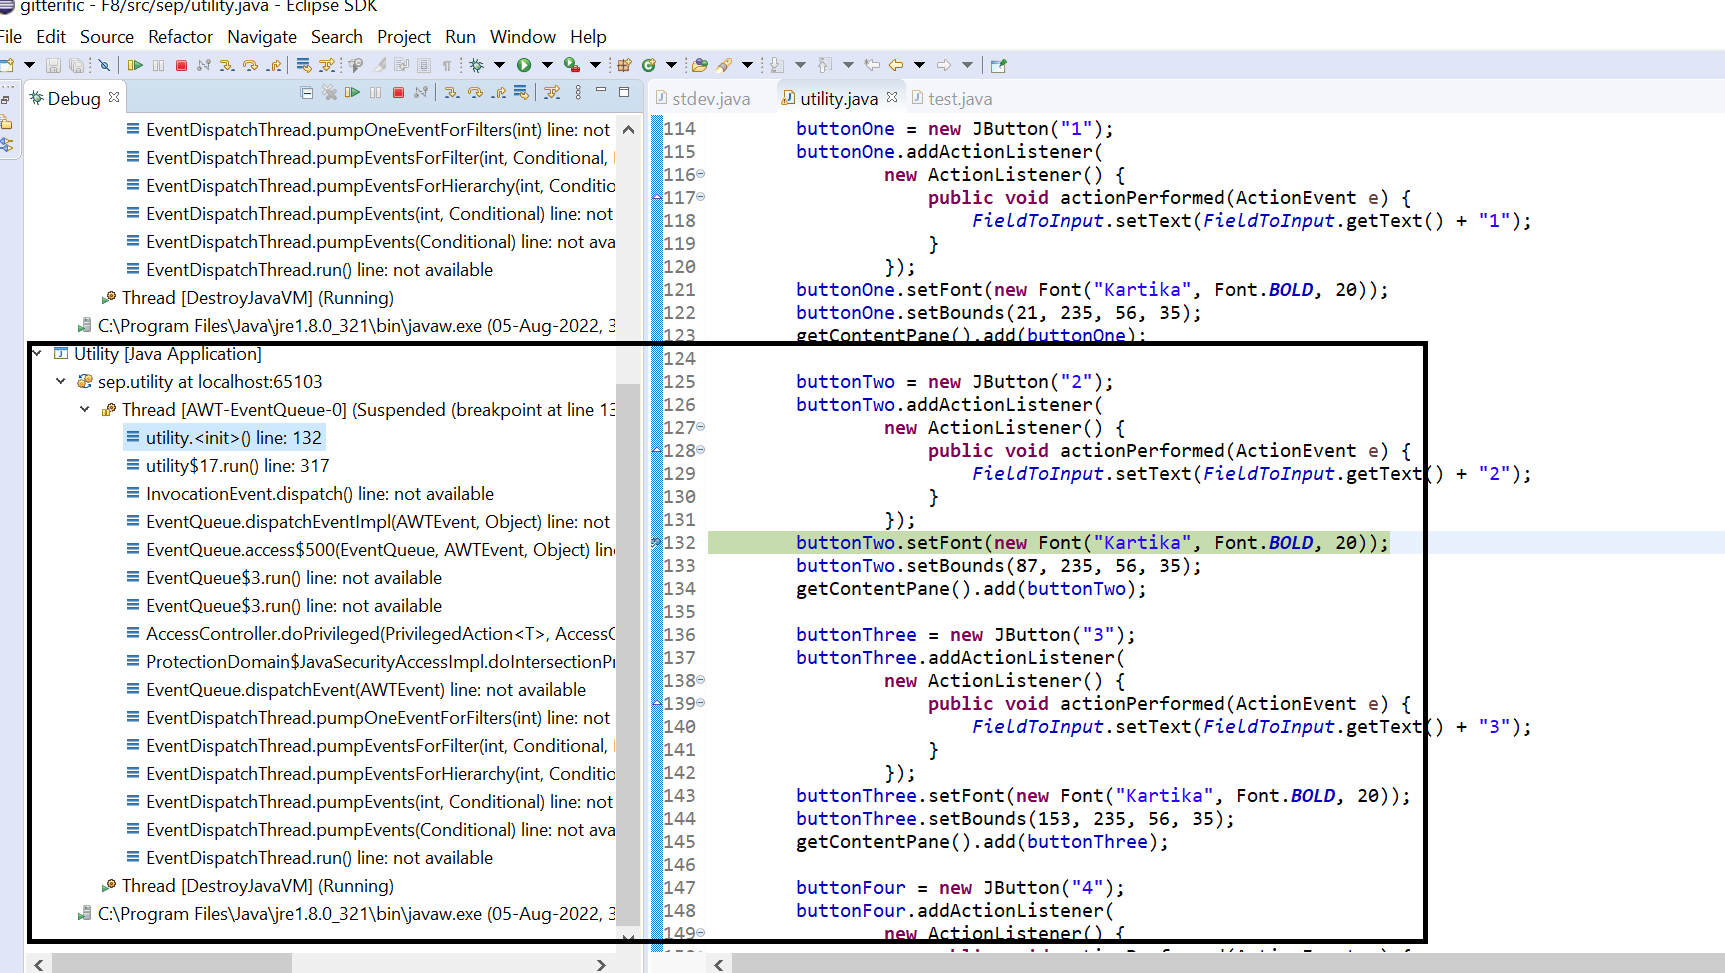
\includegraphics[width=8cm, height=2.5cm]{images/UtilityDebugger.png} 
  \end{center}
  \caption{Debugger snapshot}
\end{figure}

\subsection{\Large Advantages}

\begin{itemize}
    \item There is an option of event based breakpoints.
    \item We can modify the program by using debugger to make it more efficient and make it free from errors.
    \item The variables value can be changed at any time while debugging the code.

\end{itemize}

\subsection{\Large Disadvantages}
\begin{itemize}
    \item It is a difficult task to debug real time programs as it is involving huge lines of code.
    \item Debugging can be time taking as it is testing each line of code.
\end{itemize}

\section{\Large \vspace{0.2 cm}Quality Attributes for the source code }


\subsection{\Large\vspace{0.2 cm}Correctness}
Here the results are correct and more accurate as the values are precise. The source code for the function is tested with all the possible values.

\subsection{\Large \vspace{0.2 cm}Maintainablity}
The program is split into several functions which make it more easier to maintain the source code. In addition to this, necessary comments have been addded to make it more maintainable.



\subsection{\Large \vspace{0.2 cm}Robustness}
The program is handling various errors and exceptions which can occur while users are entering inputs and taking out results. 

\subsection{\Large \vspace{0.2 cm}Time-efficient}
Suitable breakpoints have been chosen for debugging the code which results in time-efficiency.

\subsection{\Large \vspace{0.2 cm}Usability}
The program is user-friendly as we have used the "Graphical user-interface" for taking inputs from the user.

\pagebreak

\section{\Large \vspace{0.1 cm}Checkstyle}

\subsection{\Large \vspace{0.1 cm}Description}
Checkstyle is a tool that automatically checks the Java source code  against a configurable set of rules. It helps the programmers to write Java code that sticks and follows a coding standard.


\begin{figure}[h!]
\begin{center}
  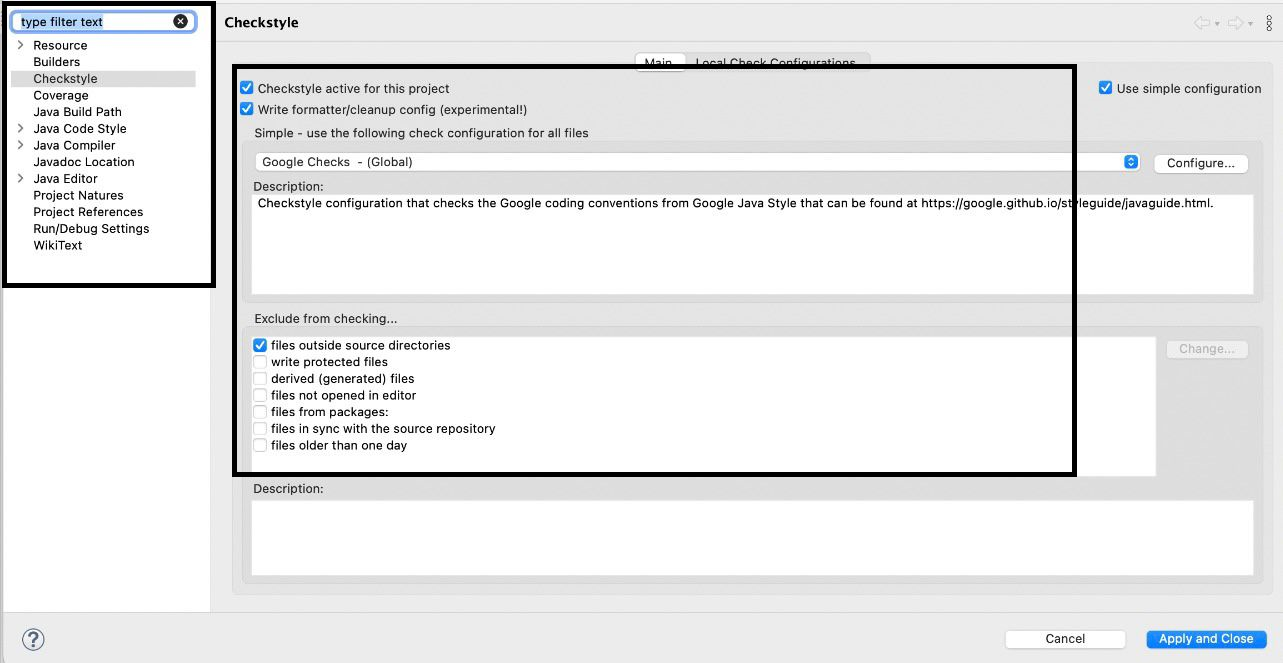
\includegraphics[width=5cm, height=2cm]{images/Activating Checkstyle tool.png}
  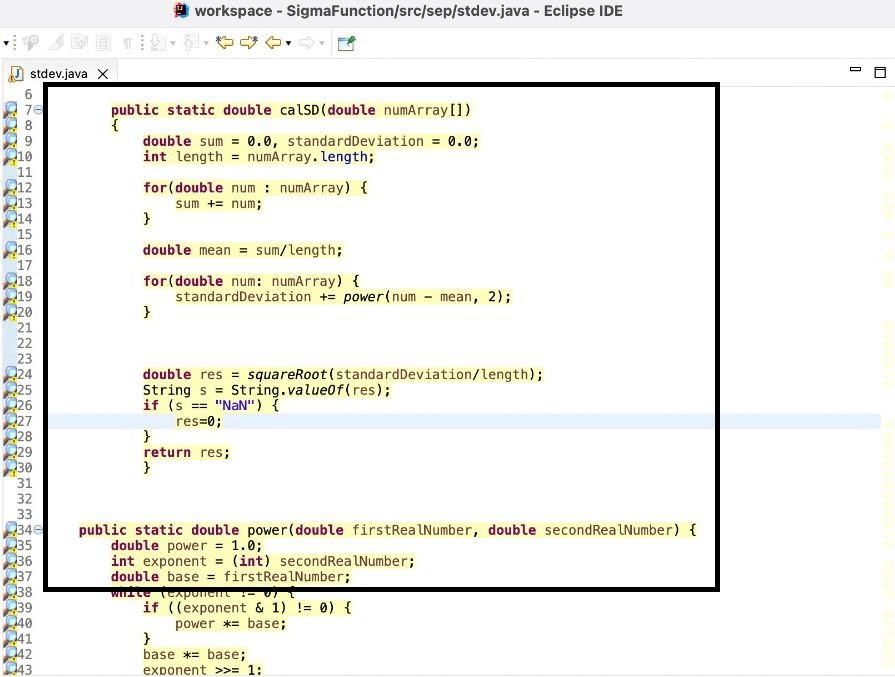
\includegraphics[width=5cm, height=2cm]{images/Applying checkStyle.jpeg}
  \end{center}
  \caption{Checkstyle Activation and Application}
\end{figure}



\subsection{\Large Advantages}

\begin{itemize}
    \item Checkstyle can check many things in the Java source code. From checking the code layout to the code formatting, it is handling everything.
    \item It has ability to create own rules for handling Java source code. Also, it can support any coding standard.
    \item Checkstyle is portable as it is easy to switch between different IDEs. In addition to this, it can find class design problems and method design problems.

\end{itemize}

\subsection{\Large Disadvantages}
\begin{itemize}
    \item It does not support any auto correct features to check any invalid coding standards.
    \item All the identifiers and keywords should be written in ASCII format only.
    \item Checkstyle tool is used only to check the format of the code and not the correctness of the code.
\end{itemize}









\begin{thebibliography}{9}
\bibitem{Debugger} 
Debugger
\\\texttt{https://www.techtarget.com/searchsoftwarequality/definition/debugging}

\bibitem{Checkstyle}
Checkstyle
\\\texttt{https://checkstyle.sourceforge.io/}



\end{thebibliography}



\end{document}